%% ------------------------------------------------------------------- %%
%% ------------------------------------------------------------------- %%
%% ------------------------------------------------------------------- %%
%% ------------------------------------------------------------------- %%
\chapter{Resultados}
\label{cap:resultados}

\lhead{\emph{Resultados}} 

%% ------------------------------------------------------------------- %%
%% ------------------------------------------------------------------- %%
%% ------------------------------------------------------------------- %%
%% ------------------------------------------------------------------- %%
%% ------------------------------------------------------------------- %%
%% ------------------------------------------------------------------- %%

%% -------------------------------------------------------------------- %%
%% -------------------------------------------------------------------- %%



En la Tabla \ref{tab:results}, presentamos el \textit{accuracy, f1 score, precision} y \textit{recall} de cada base de datos (\textit{allele}). Como podemos ver, en todos los casos superamos el 0.9 de \textit{accuracy}, esto valida la propuesta y da origen a seguir trabajando en mejorar la propuesta. \\

Luego, en la Figura \ref{fig:result}, presentamos el \textit{accuracy} obtenido durante el entrenamiento de cada base de datos con el conjunto de muestras de entrenamiento y validación. En este caso, utilizamos el 20\% de las muestras de entrenamiento como validación. Como podemos ver, con solo 10 \textit{epochs},  se lograron buenos resultados. Tambien se evaluao con mas \textit{epochs}, pero los resultados no mejoraron.

\begin{table}[]
	\centering
	\caption{Resultados obtenidos en cada base de datos. }
	\label{tab:results}
	\setlength{\tabcolsep}{0.8em} % for the horizontal padding
	{\renewcommand{\arraystretch}{1.3}% for the vertical padding
		\begin{tabular}{lllll}
			\hline
			\textit{\textbf{Allele}} & \textit{\textbf{Accuracy}} & \textit{\textbf{F1 score}} & \textit{\textbf{Precision}} & \textit{\textbf{Recall}} \\
			\hline
			A*01:01                  & 0.978                      & 0.917                      & 0.982                       & 0.887                    \\
			A*0201                   & 0.962                      & 0.956                      & 0.965                       & 0.948                    \\
			A*02:03                  & 0.992                      & 0.979                      & 0.994                       & 0.969                    \\
			A*31:01                  & 0.980                      & 0.968                      & 0.989                       & 0.951                    \\
			B*44:02                  & 0.991                      & 0.981                      & 0.968                       & 0.997                    \\
			B*44:03                  & 0.992                      & 0.987                      & 0.995                       & 0.980                   
		\end{tabular}
	}
\end{table}

\begin{figure}[H]
	\centering
	\subfigure[A*01:01]{\label{fig:a}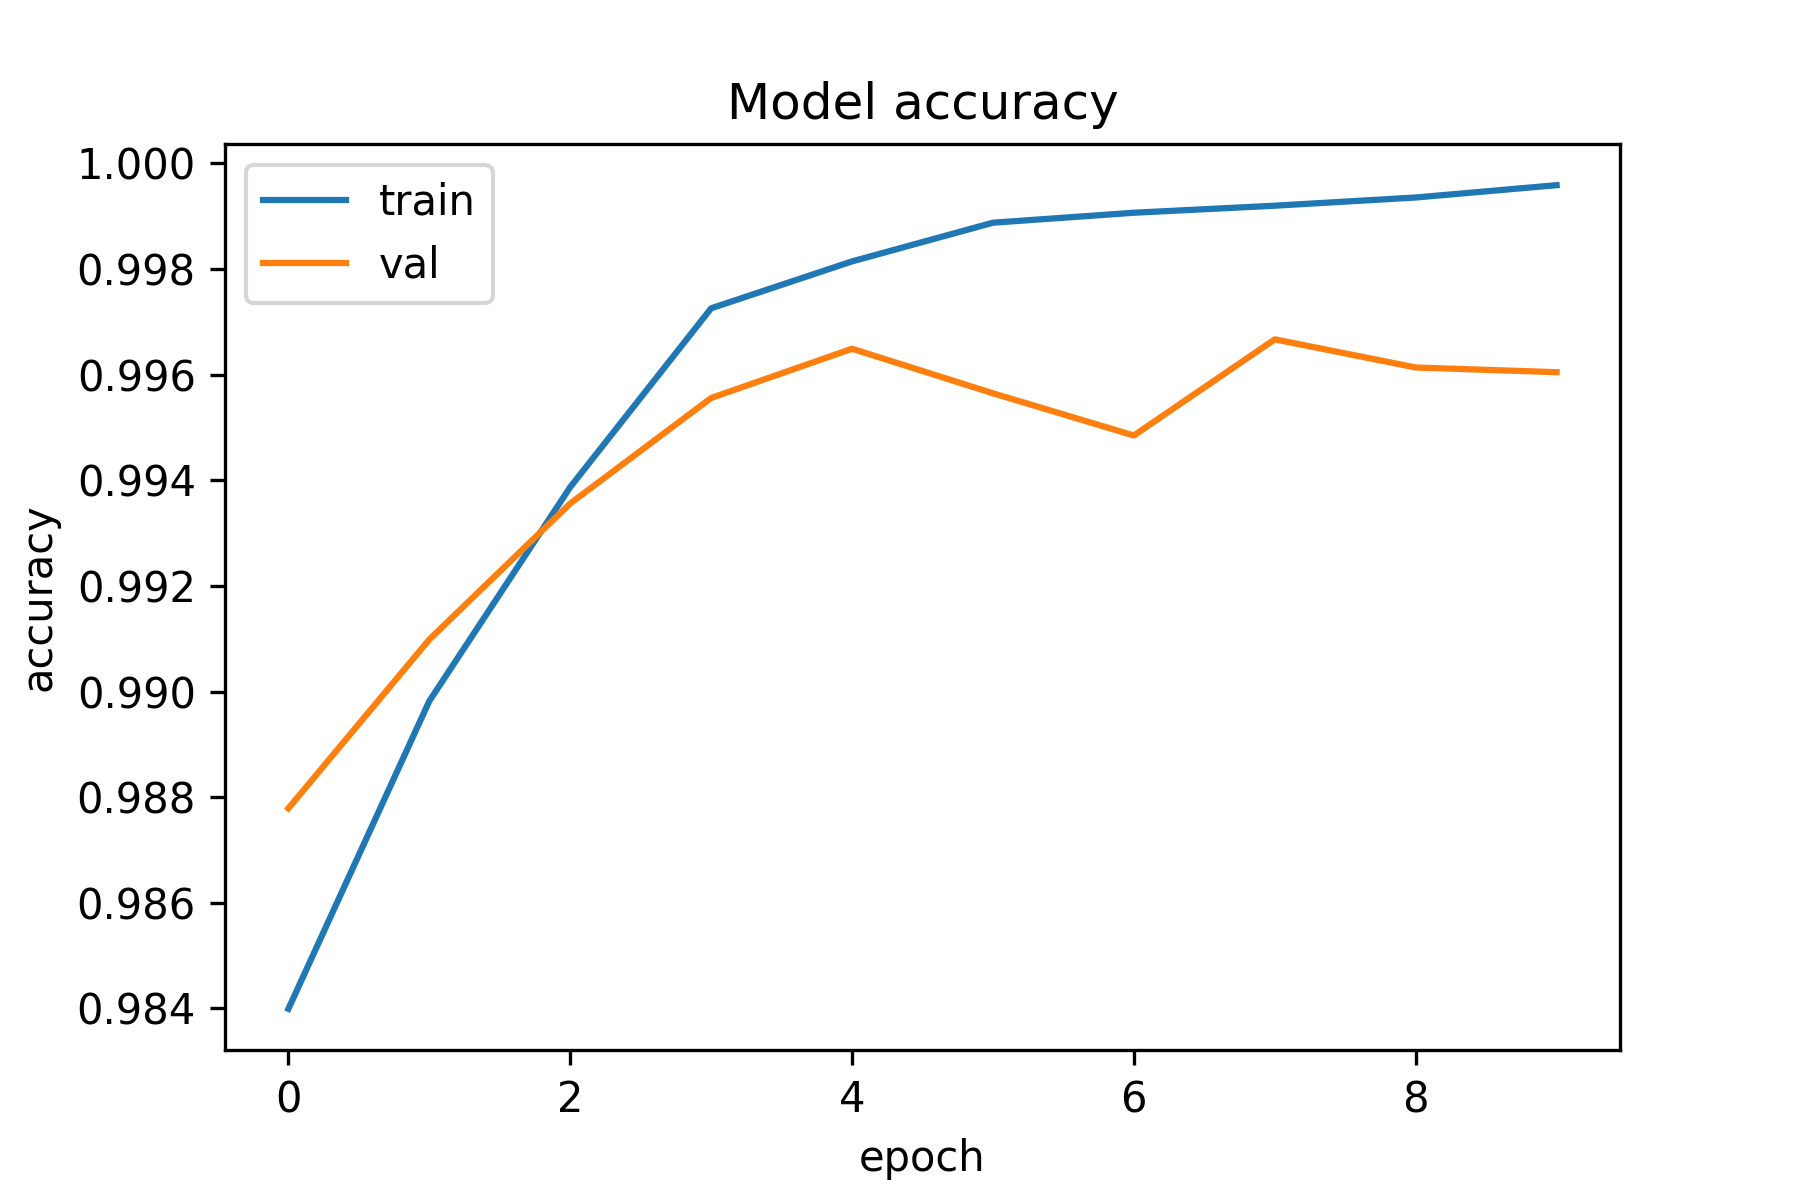
\includegraphics[width=0.45\textwidth]{img/neoantigen/acc_A0203}}
	\subfigure[A*02:01]{\label{fig:b}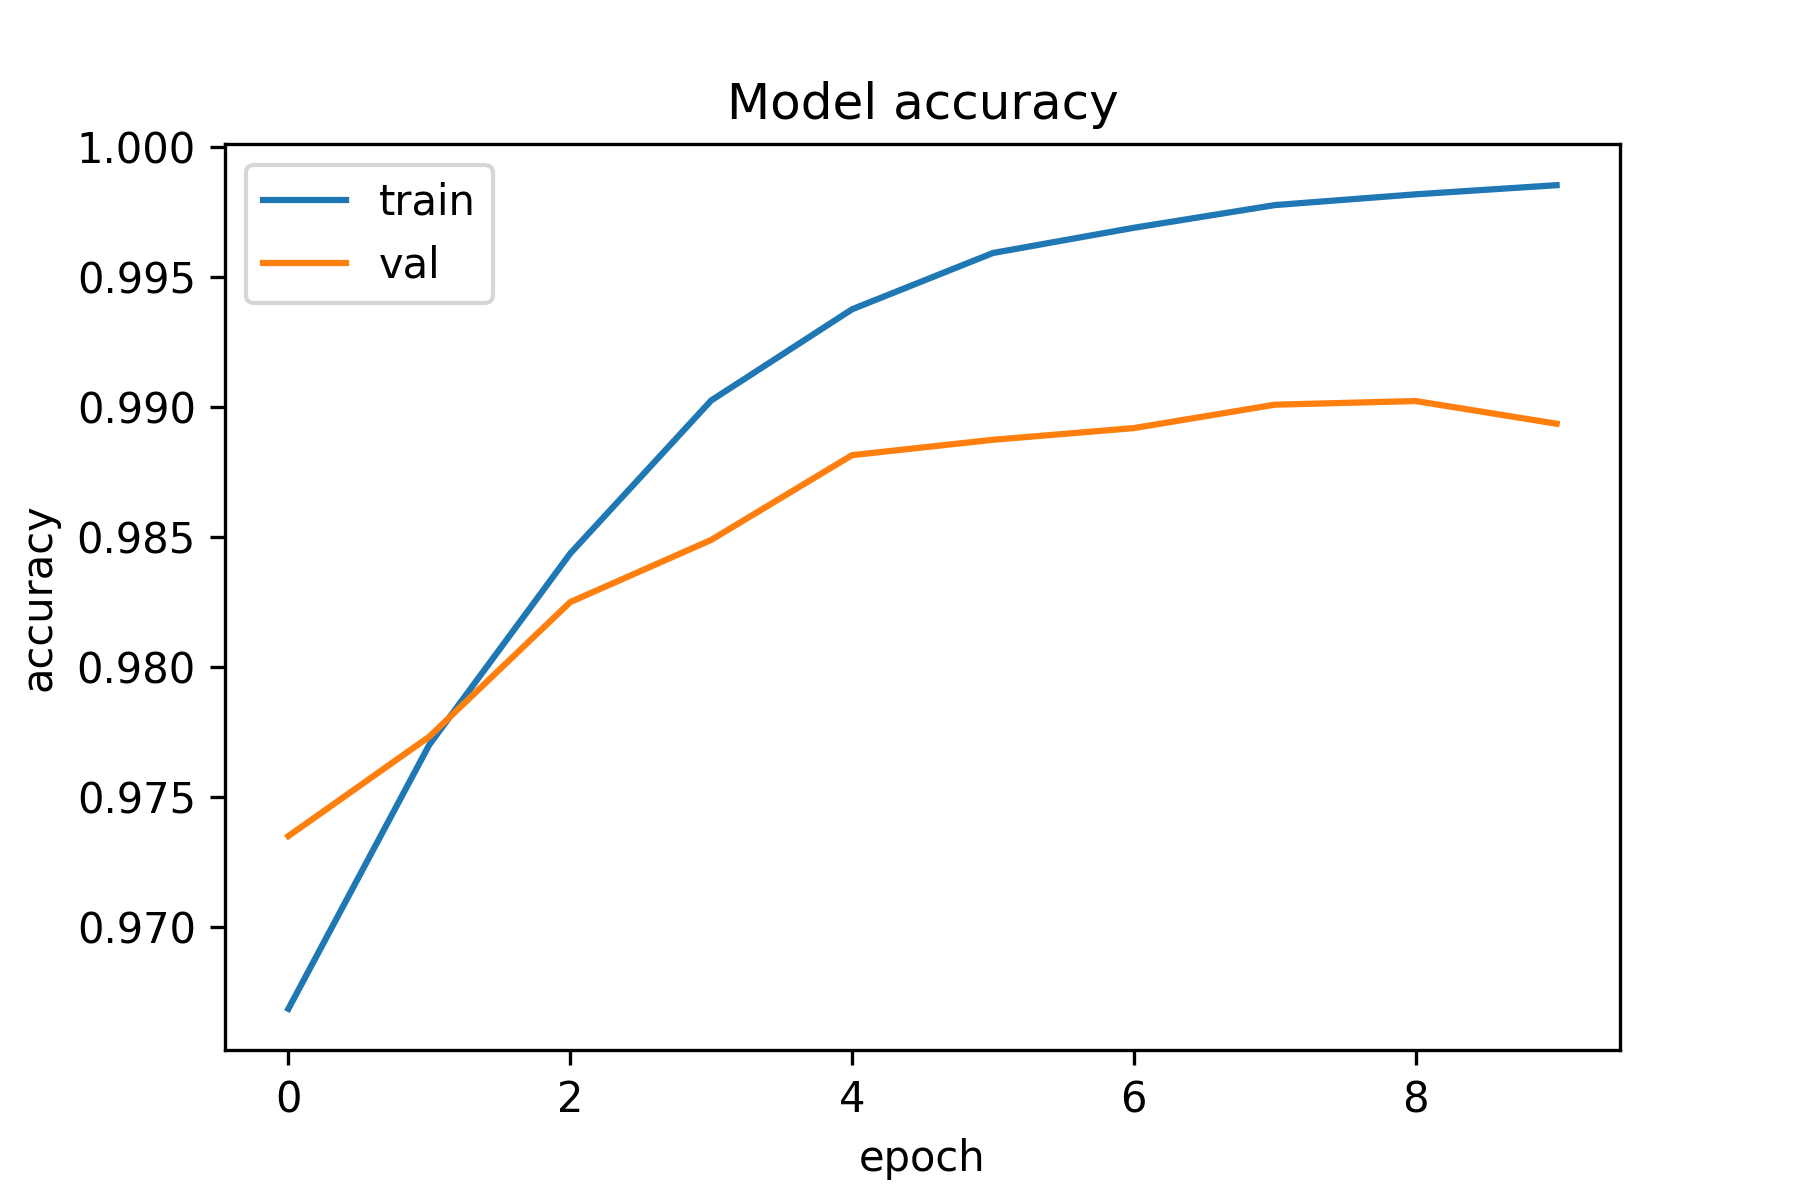
\includegraphics[width=0.45\textwidth]{img/neoantigen/acc_A0201}}
	\subfigure[A*02:03]{\label{fig:a}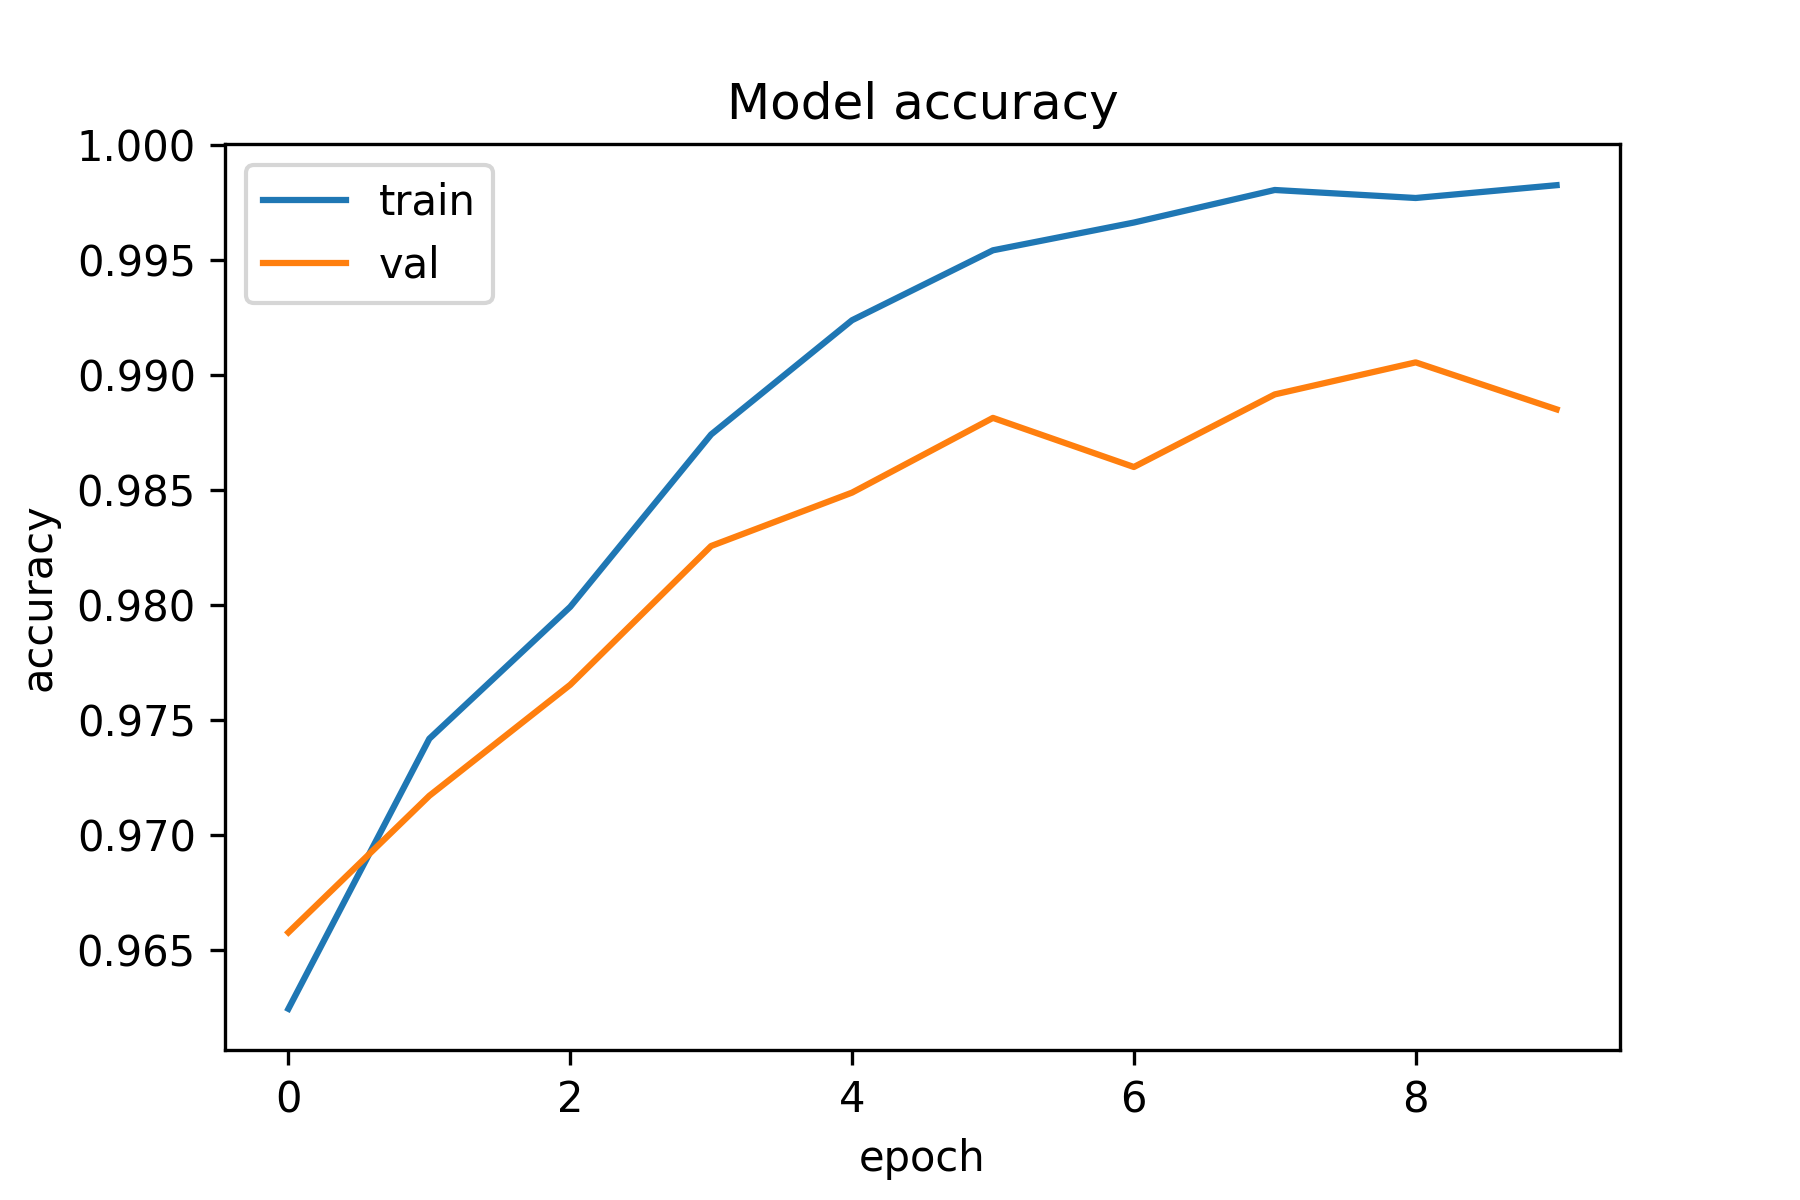
\includegraphics[width=0.45\textwidth]{img/neoantigen/acc_A0101}}
	\subfigure[A*31:01]{\label{fig:b}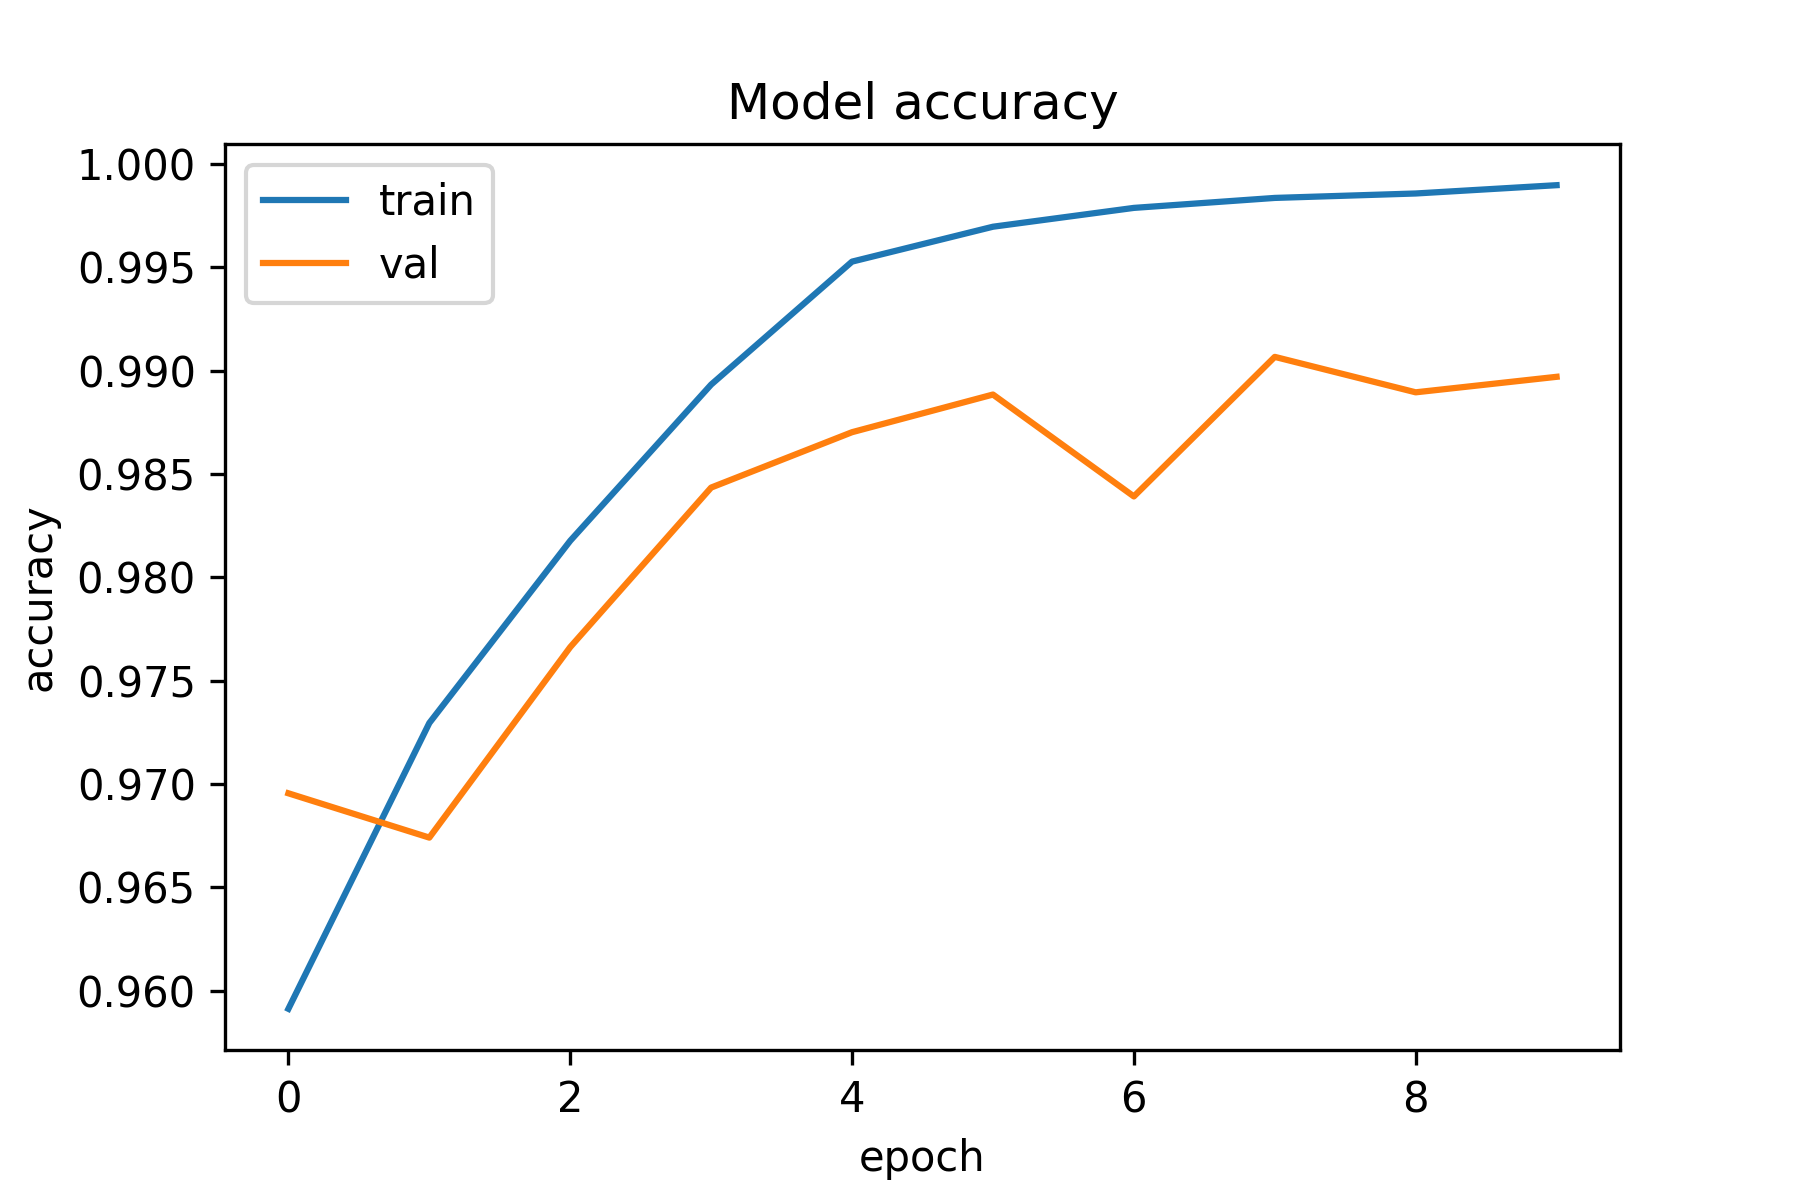
\includegraphics[width=0.45\textwidth]{img/neoantigen/acc_A3101}}
	\subfigure[B*44:02]{\label{fig:a}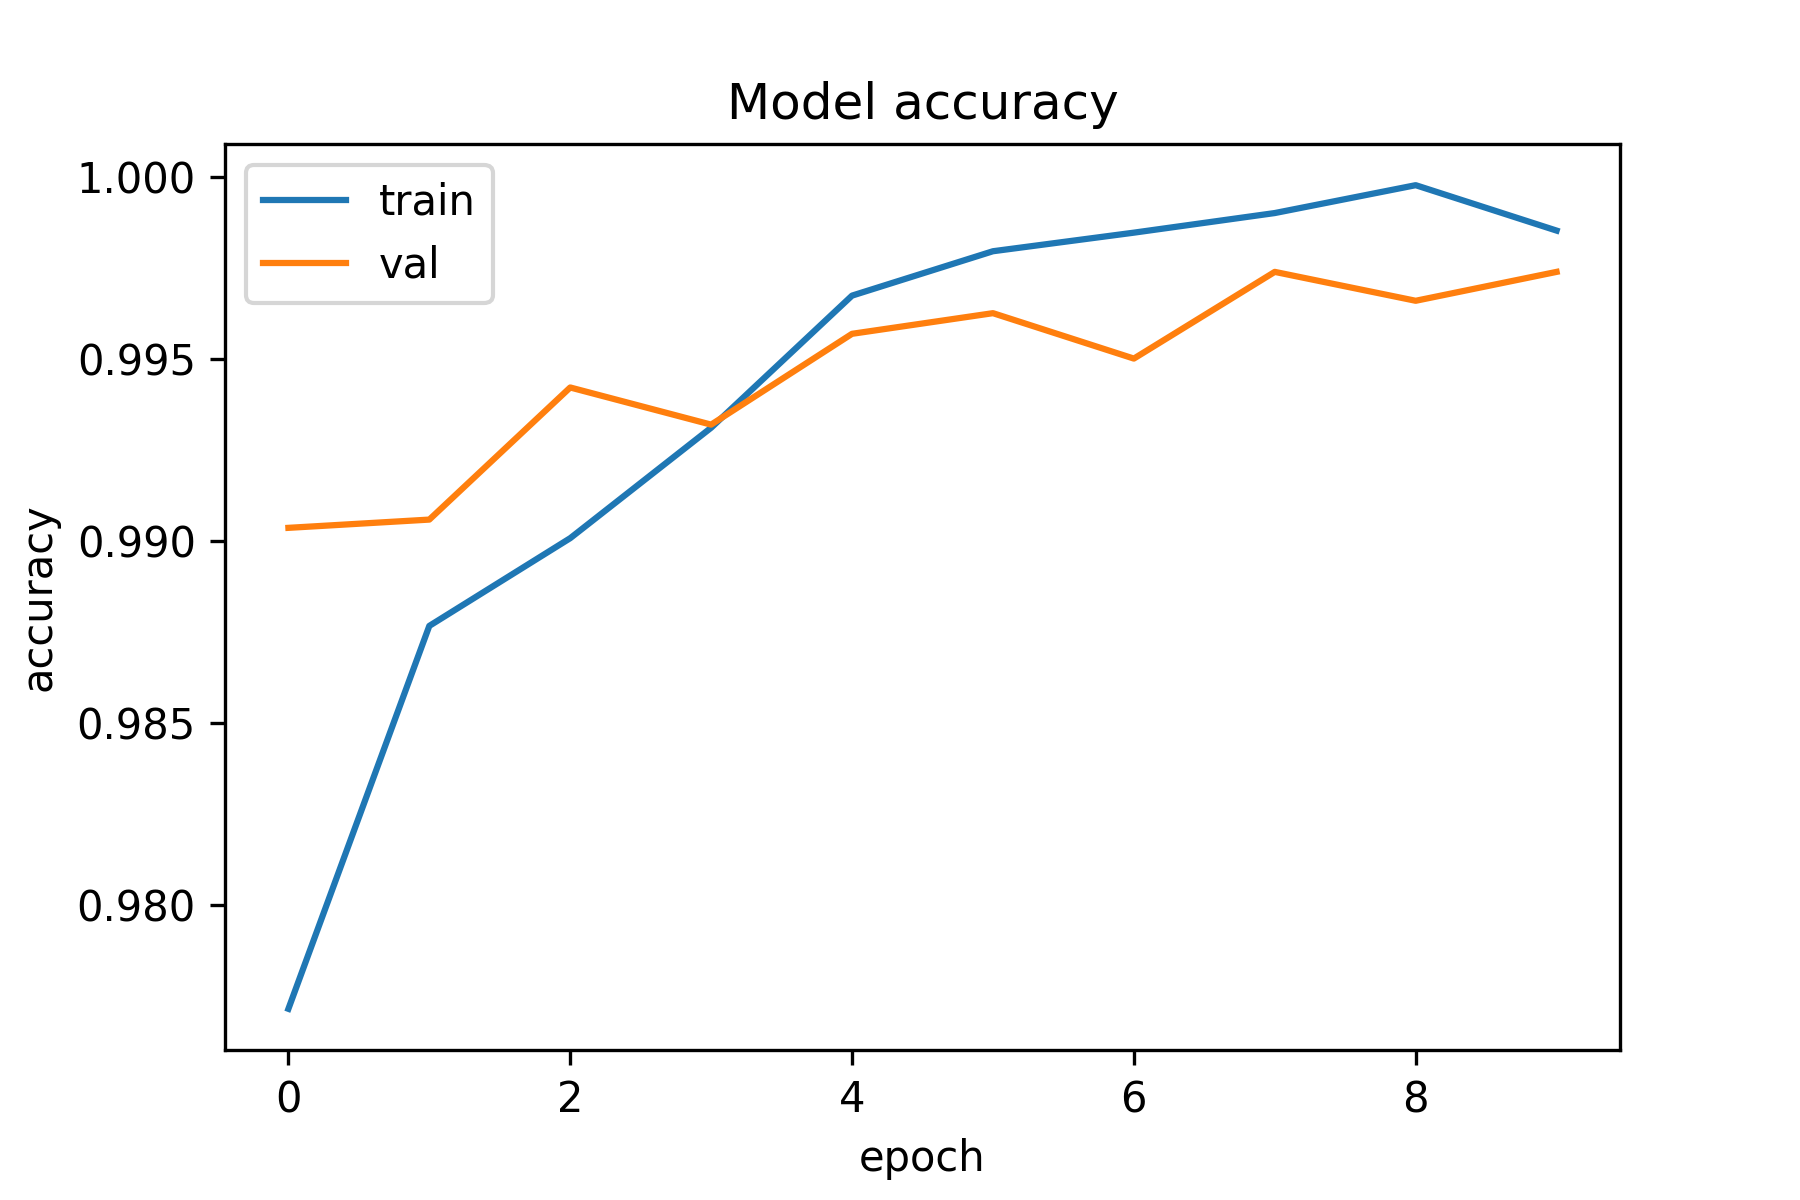
\includegraphics[width=0.45\textwidth]{img/neoantigen/acc_B4402}}
	\subfigure[B*44:03]{\label{fig:b}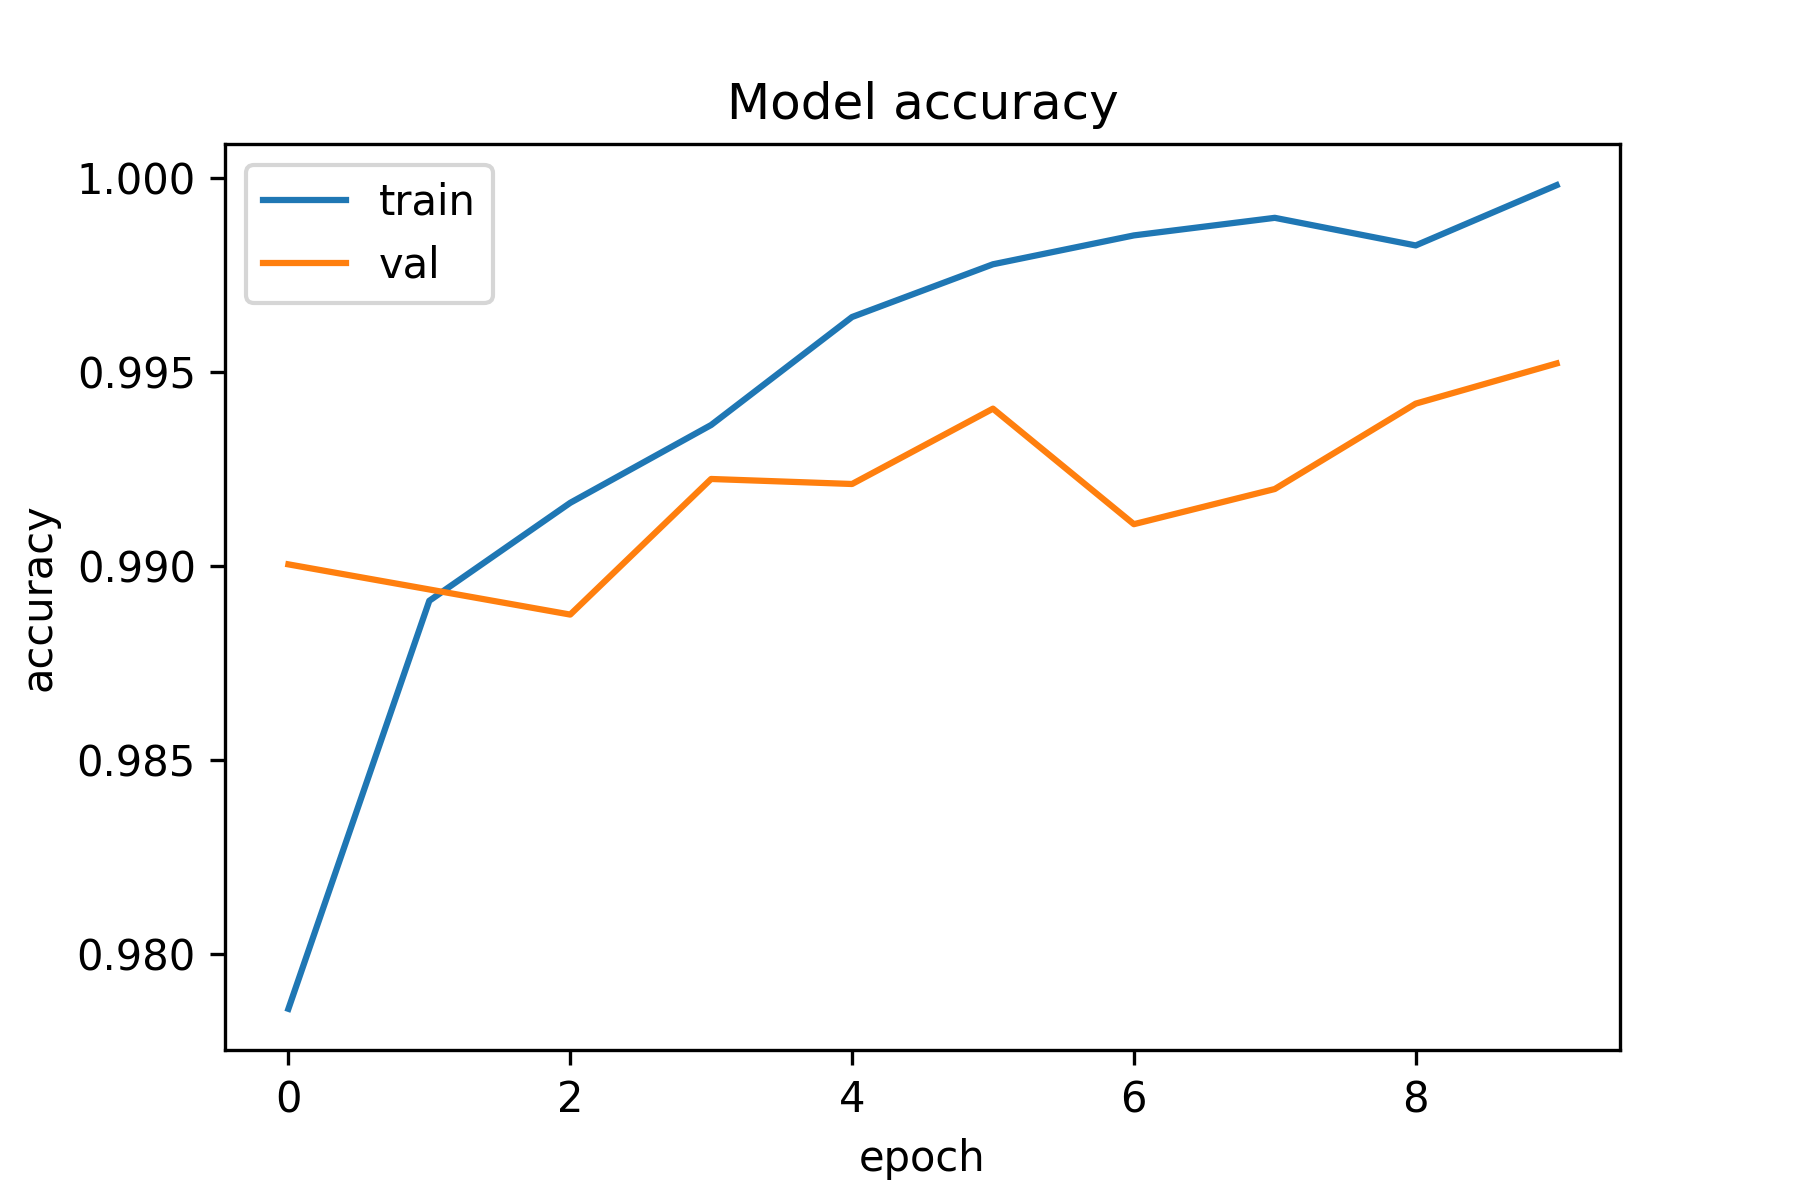
\includegraphics[width=0.45\textwidth]{img/neoantigen/acc_B4403}}
	
	
	\caption{\textit{Accuracy} durante cada \textit{epoch}, para cada base de datos. Las bases de datos representan las células HLA A*01:01, A*02:01, A*02:03, A*31:01, B*44:02 y B*44:03.}
	\label{fig:result}
\end{figure}